% ============================================================================
\section{Introduction}
\label{sec:intro}
% ============================================================================

Multi-teacher on-policy distillation (MOPD) provides a practical way to
combine capabilities in one language model. The student generates responses,
and each response is scored by the teacher assigned to its task
\citep{ma2026mopdmultiteacheronpolicydistillation}. This allows specialist
teachers to be developed separately and their feedback to be combined during
student training. The same approach can add a new capability while using an
earlier model as a teacher to preserve existing ones
\citep{liu2026instella}. Once the teachers are available, a recurring
engineering question is how to divide the student's training budget among
their tasks.

Existing recipes address several parts of this problem. Open-MOPD adjusts
loss weights to compensate for response-length imbalance and to emphasize
domains with larger teacher--student gaps
\citep{gao2026openmopddiagnosingfixingcapability}. D$^3$-MOPD changes the
sampling mixture using the remaining gap and its recent rate of decrease
\citep{sun2026d3mopd}. These approaches make the allocation responsive to
task balance and learning progress. They also motivate a complementary
question: for a chosen balance of task objectives, how many samples are
needed to obtain a reliable update from each task?

Consider two equally weighted tasks. One gives similar gradients across
micro-batches, while the other gives gradients that fluctuate widely with
the sampled prompts and responses. Equal counts spend the same computation
on both estimates even though the second is less precise. Giving the second
task more micro-batches can make the combined update more reliable. Its
objective weight can stay the same: first average the gradients within each
task, then combine those averages with the chosen weights. Task importance
and the amount of computation used to estimate its update are separate
choices.

This distinction remains useful with dense distillation. MOPD already
supports a teacher top-$k$ loss, and recent methods improve how retained
tokens and the distribution tail contribute to supervision
\citep{ma2026mopdmultiteacheronpolicydistillation,huang2026tailaware}.
Even when all retained-token contributions are computed at a fixed prefix,
different prompts and student rollouts still yield different gradients.
The relevant signal for allocation is therefore the variability of the
actual training gradient. Teacher loss alone does not describe that
variability: two tasks can have similar losses but different gradient
directions and response lengths.

We propose Gradient-Preconditioned Adaptive Sampling (GPAS), which allocates
micro-batches using the gradient variation observed during ordinary MOPD
training. GPAS measures this variation after the optimizer's coordinate
scaling. This matters because a fluctuation has a larger effect on an update
when the optimizer amplifies the coordinates in which it occurs. With fixed
task weights, the resulting rule gives each task a count proportional to
its weighted preconditioned standard deviation. A cost-aware mode also
uses measured running time, allowing the same scheduler to target
efficiency per step or per GPU hour.

\begin{figure}[t]
    \centering
    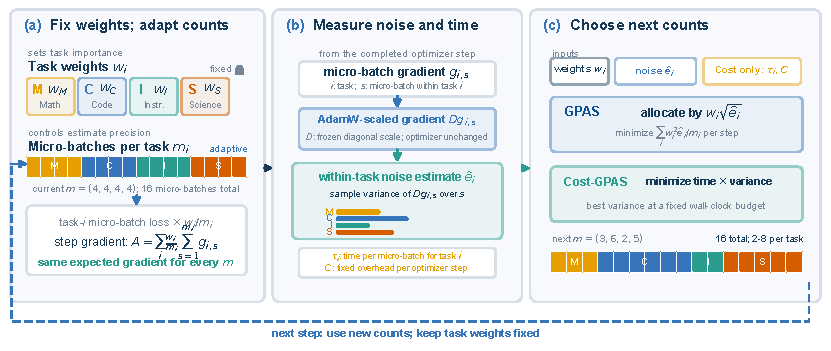
\includegraphics[width=\linewidth]{figures/gpas_main_figure.pdf}
    \caption{GPAS separates task importance from computation.
    Task means are combined with fixed weights $w$, while counts $m$ adapt
    to the variation of ordinary dense-distillation gradients. The optimizer's
    pre-step scaling $D$ determines how those fluctuations affect the update.
    Observed noise and running time guide the next allocation. The task
    profiles are schematic.}
    \label{fig:gpas_overview}
\end{figure}

Our study follows this practical sequence: compare learning curves and
per-domain capability, examine where GPAS spends computation, and measure
the contributions of optimizer scaling and running time. All core allocation
comparisons use the same existing top-$k$ loss. A second dense loss tests
the same scheduling idea with tail-aware supervision.
\missing{Summarize the main efficiency and capability results and the
allocation pattern that explains them.}

The paper makes three contributions:
\begin{itemize}
    \item a practical separation of task weights and micro-batch counts for
    MOPD, so computation can adapt while each task retains its intended
    contribution to the expected gradient;
    \item an optimizer-aware allocation method that reuses micro-batch
    gradients, with a cost-aware mode based on measured task time;
    \item a four-domain study relating training efficiency and capability
    integration to gradient variability, learning progress, and the
    allocation of computation.
\end{itemize}
